\section{Métodos de apoio à decisão}
\label{sec:metodos}

A expressão \textit{framework} foi identificada em 96 dos 104 registros. \textit{Decision support} e BIM aparecem em 26 registros cada, seguidos de otimização em 18, pontuação em 17 e custo do ciclo de vida em 13. Entre os métodos formalmente nomeados, foram identificados AHP em cinco registros, TOPSIS em quatro, ANP e MCDM em três registros cada e \textit{Bayesian Best-Worst Method} em um registro. O Gráfico~\ref{fig:metodos} separa abordagens gerais e métodos estruturados para facilitar a leitura.

\begin{figure}[H]
\centering
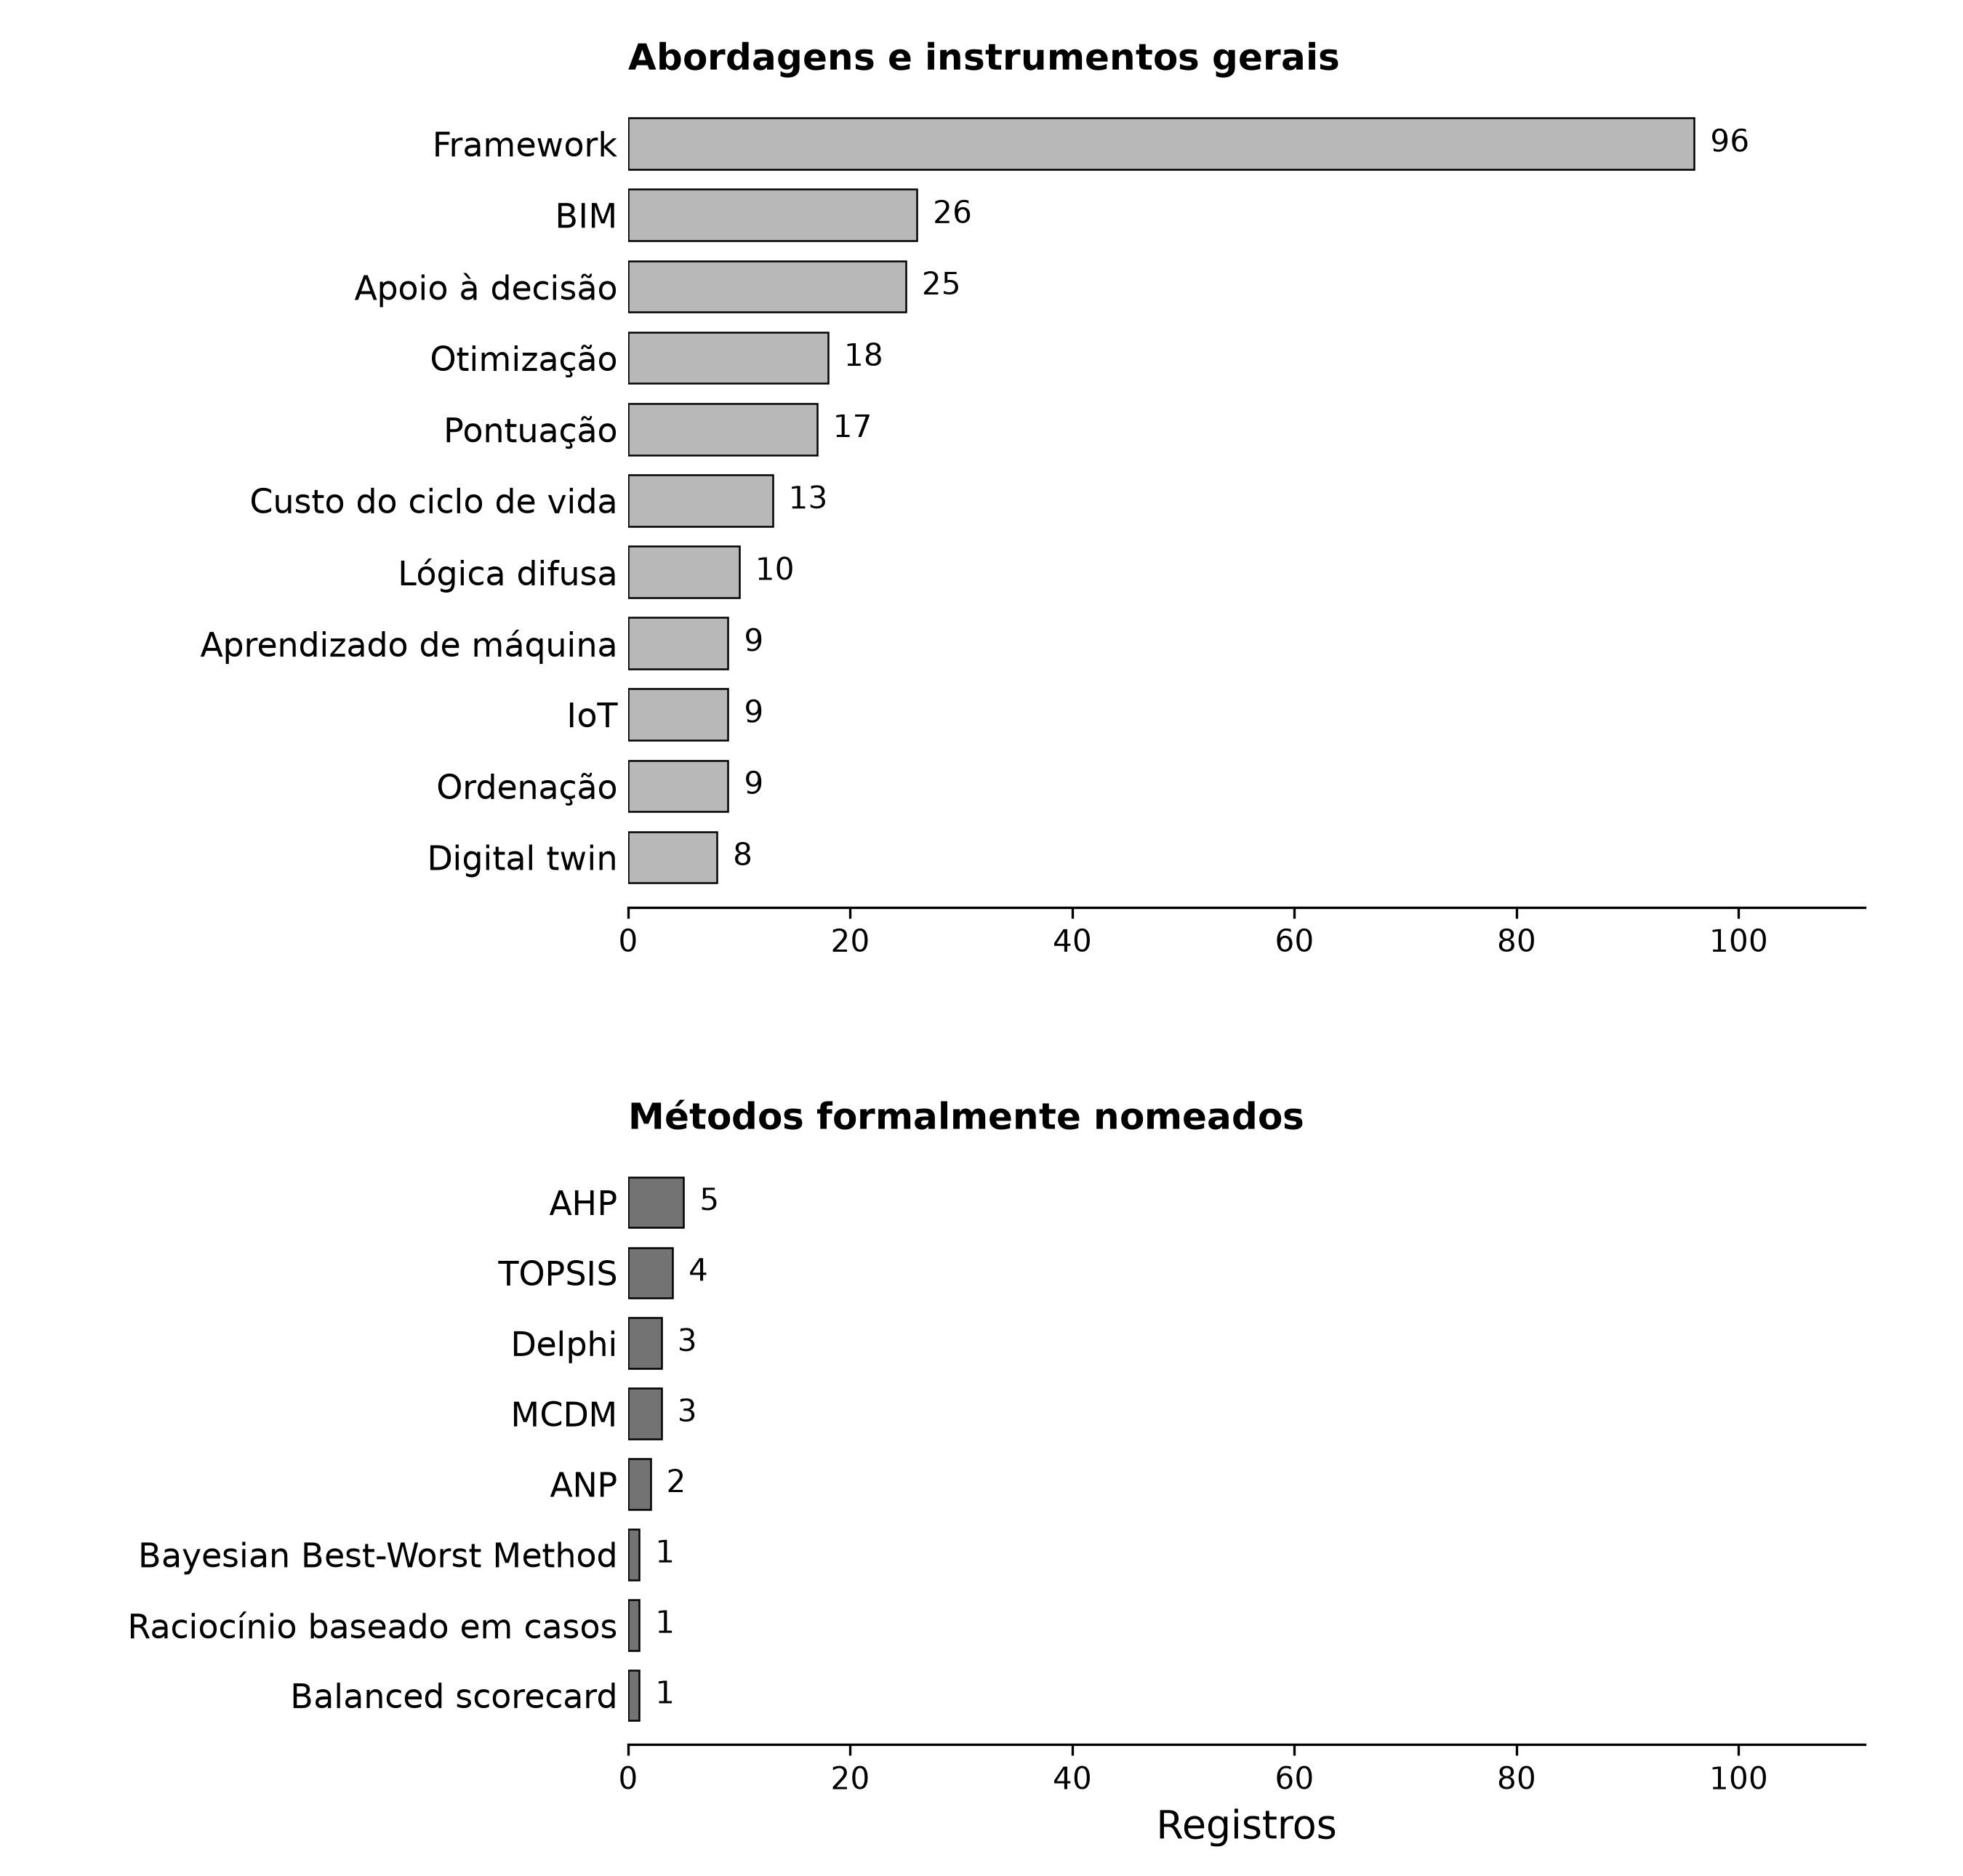
\includegraphics[width=0.95\linewidth]{figuras/figura11_metodos_mcdm_mais_frequentes_nucleo_final_104.png}
\captiongrafico{Abordagens e métodos de apoio à decisão identificados no núcleo final}
\label{fig:metodos}
\end{figure}

Os estudos do núcleo ilustram diferentes formas de estruturar a decisão. O modelo de \textcite{alfalah_frameworkeducacional_2022} combina avaliação de sustentabilidade e ANP difuso em edifícios de ensino. \textcite{naji_campusdelphi_2023} utilizam Delphi modificado para desenvolver um referencial operacional de gestão de facilidades em \textit{campus}. \textcite{masmoudi_ahptopsis_2026} integram AHP, TOPSIS e otimização na alocação de prestadores para manutenção de edifícios públicos. Em conjunto, essas aplicações mostram que os métodos podem organizar critérios técnicos, econômicos, ambientais e sociais em diferentes problemas de gestão predial.

